\chapter{Results}
\label{c:result}

\begin{figure}
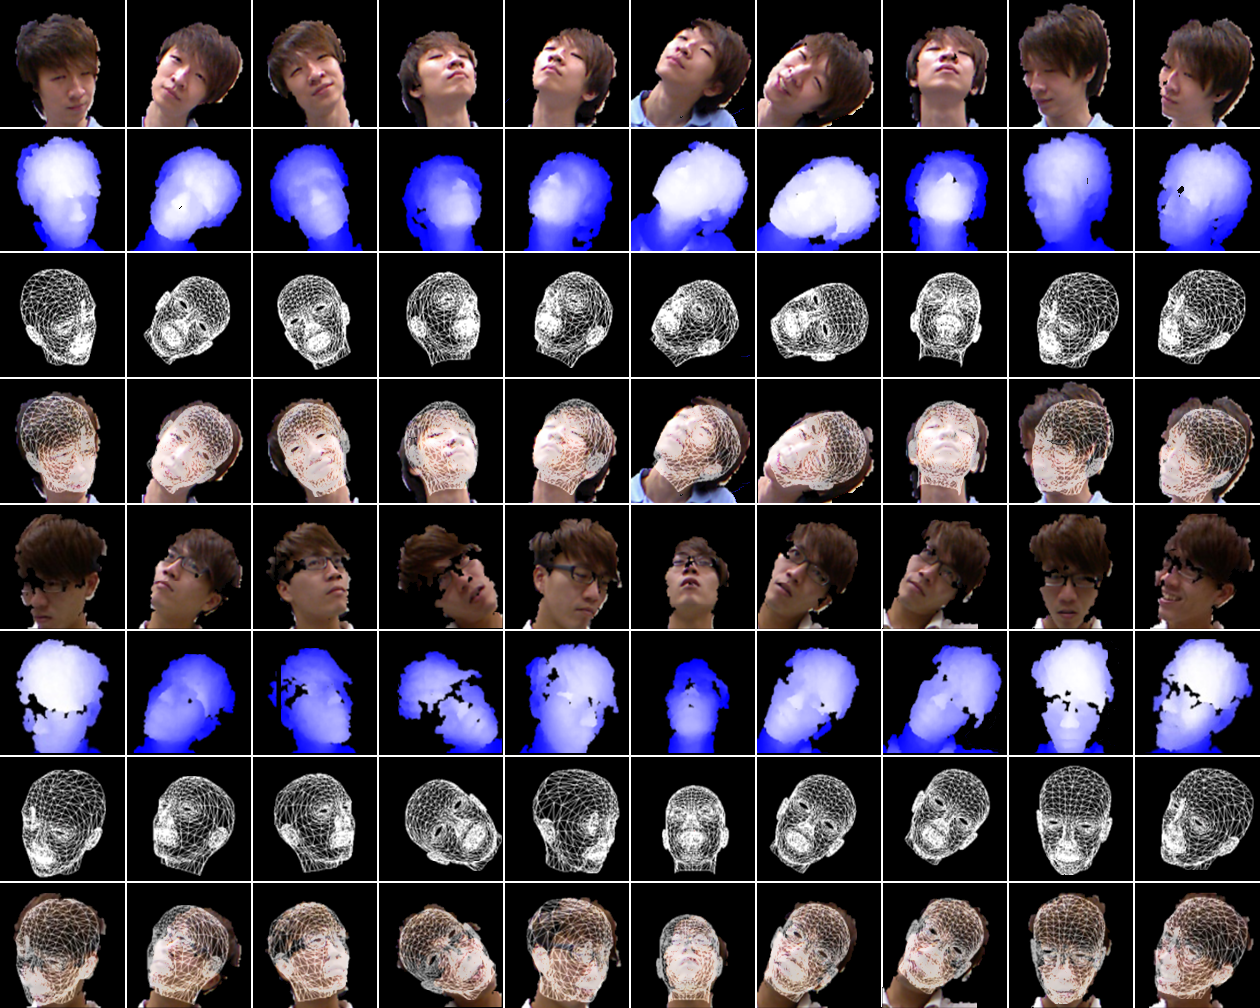
\includegraphics[width=1.0\linewidth]{./figure/m1_result.png}
\caption{The experimental results of two users for performing head pose, each one has different nose size and hair fringe. The result also shows that wearing eyeglasses will not decrease the accuracy.}
\label{f:m1 result}       % Give a unique label
\end{figure}


\begin{figure}
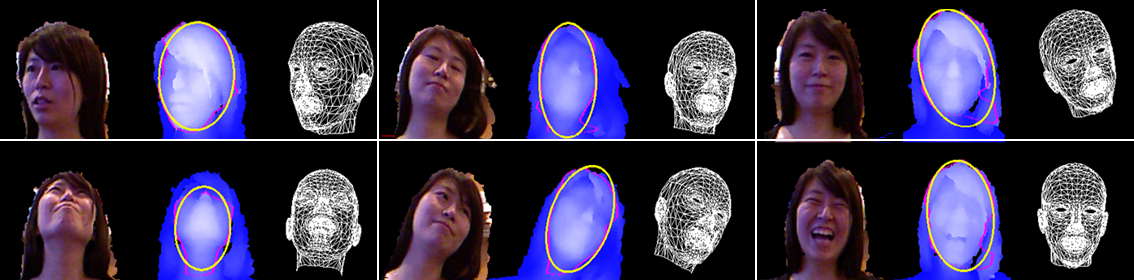
\includegraphics[width=1.0\linewidth]{./figure/m1_result_opal.png}
\caption{Results of female users are as accurate as male users in terms of yaw and pitch angles while long hair may affect the boundary detection and further decrease accuracy of roll angle estimation (left-bottom). The right-bottom picture shows that dramatic facial expression doesn’t affect the estimation.}
\label{f:m1 result girl}       % Give a unique label
\end{figure}

Figure \ref{f:m1 result} shows the results of two user who makes arbitrary poses estimated by least square solution (method 1). The first and fifth rows show what poses users make, note that our system doesn't take any advantage from these color images so that it still performs well under variation of illumination. The second and sixth tows are the depth maps captured by the 3D sensor. The third and seventh rows show the results by retarget the estimated motion vector to a virtual character. The fourth and eighth rows overlap the virtual characters with the human pose images.

In our experiments for method 1, 14 people were tested. In general, this method succeeds in estimating the head pose within the range of $\pm 50^{\circ}$ yaw, $\pm 40^{\circ}$ pitch and $\pm 70^{\circ}$ roll rotations. Comparing to state-of-the-art methods such as \cite{Breitenstein:08:RTFPEFSRI, Fanelli:11:RTHPEWRRF, fanelli_DAGM11}, although our capability on pitch and yaw angles estimating are not as good as them, it is worth mentioning that our estimation on roll angles outperforms them. However, since the nose tip position is a key element in the proposed algorithm, the estimation on yaw and pitch angles may fail once the nose is not detected successfully. In this case, manual refocusing is required. 

It is also observed from the experiments that the hair style may affect the estimation. Long hairs may interfere in the procedure of face boundaries detection and cause the decrease of accuracy in roll angle estimation (as shown in the left-bottom of Figure \ref{f:m1 result girl}). Fortunately, the estimation in yaw and pitch angles will not be affected by the hair style.

\begin{figure}
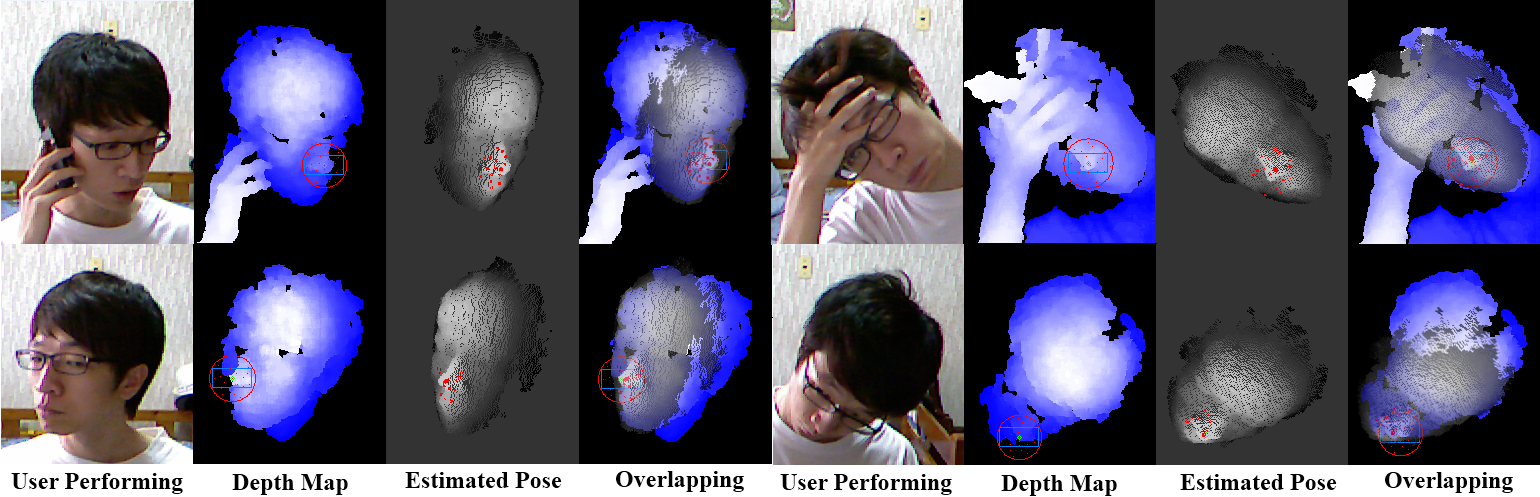
\includegraphics[width=1.0\linewidth]{./figure/m2_result_tuyu.png}
\caption{Experimental results of optimization solution.}
\label{f:m2 result tantofish}       % Give a unique label
\end{figure}

\begin{figure}
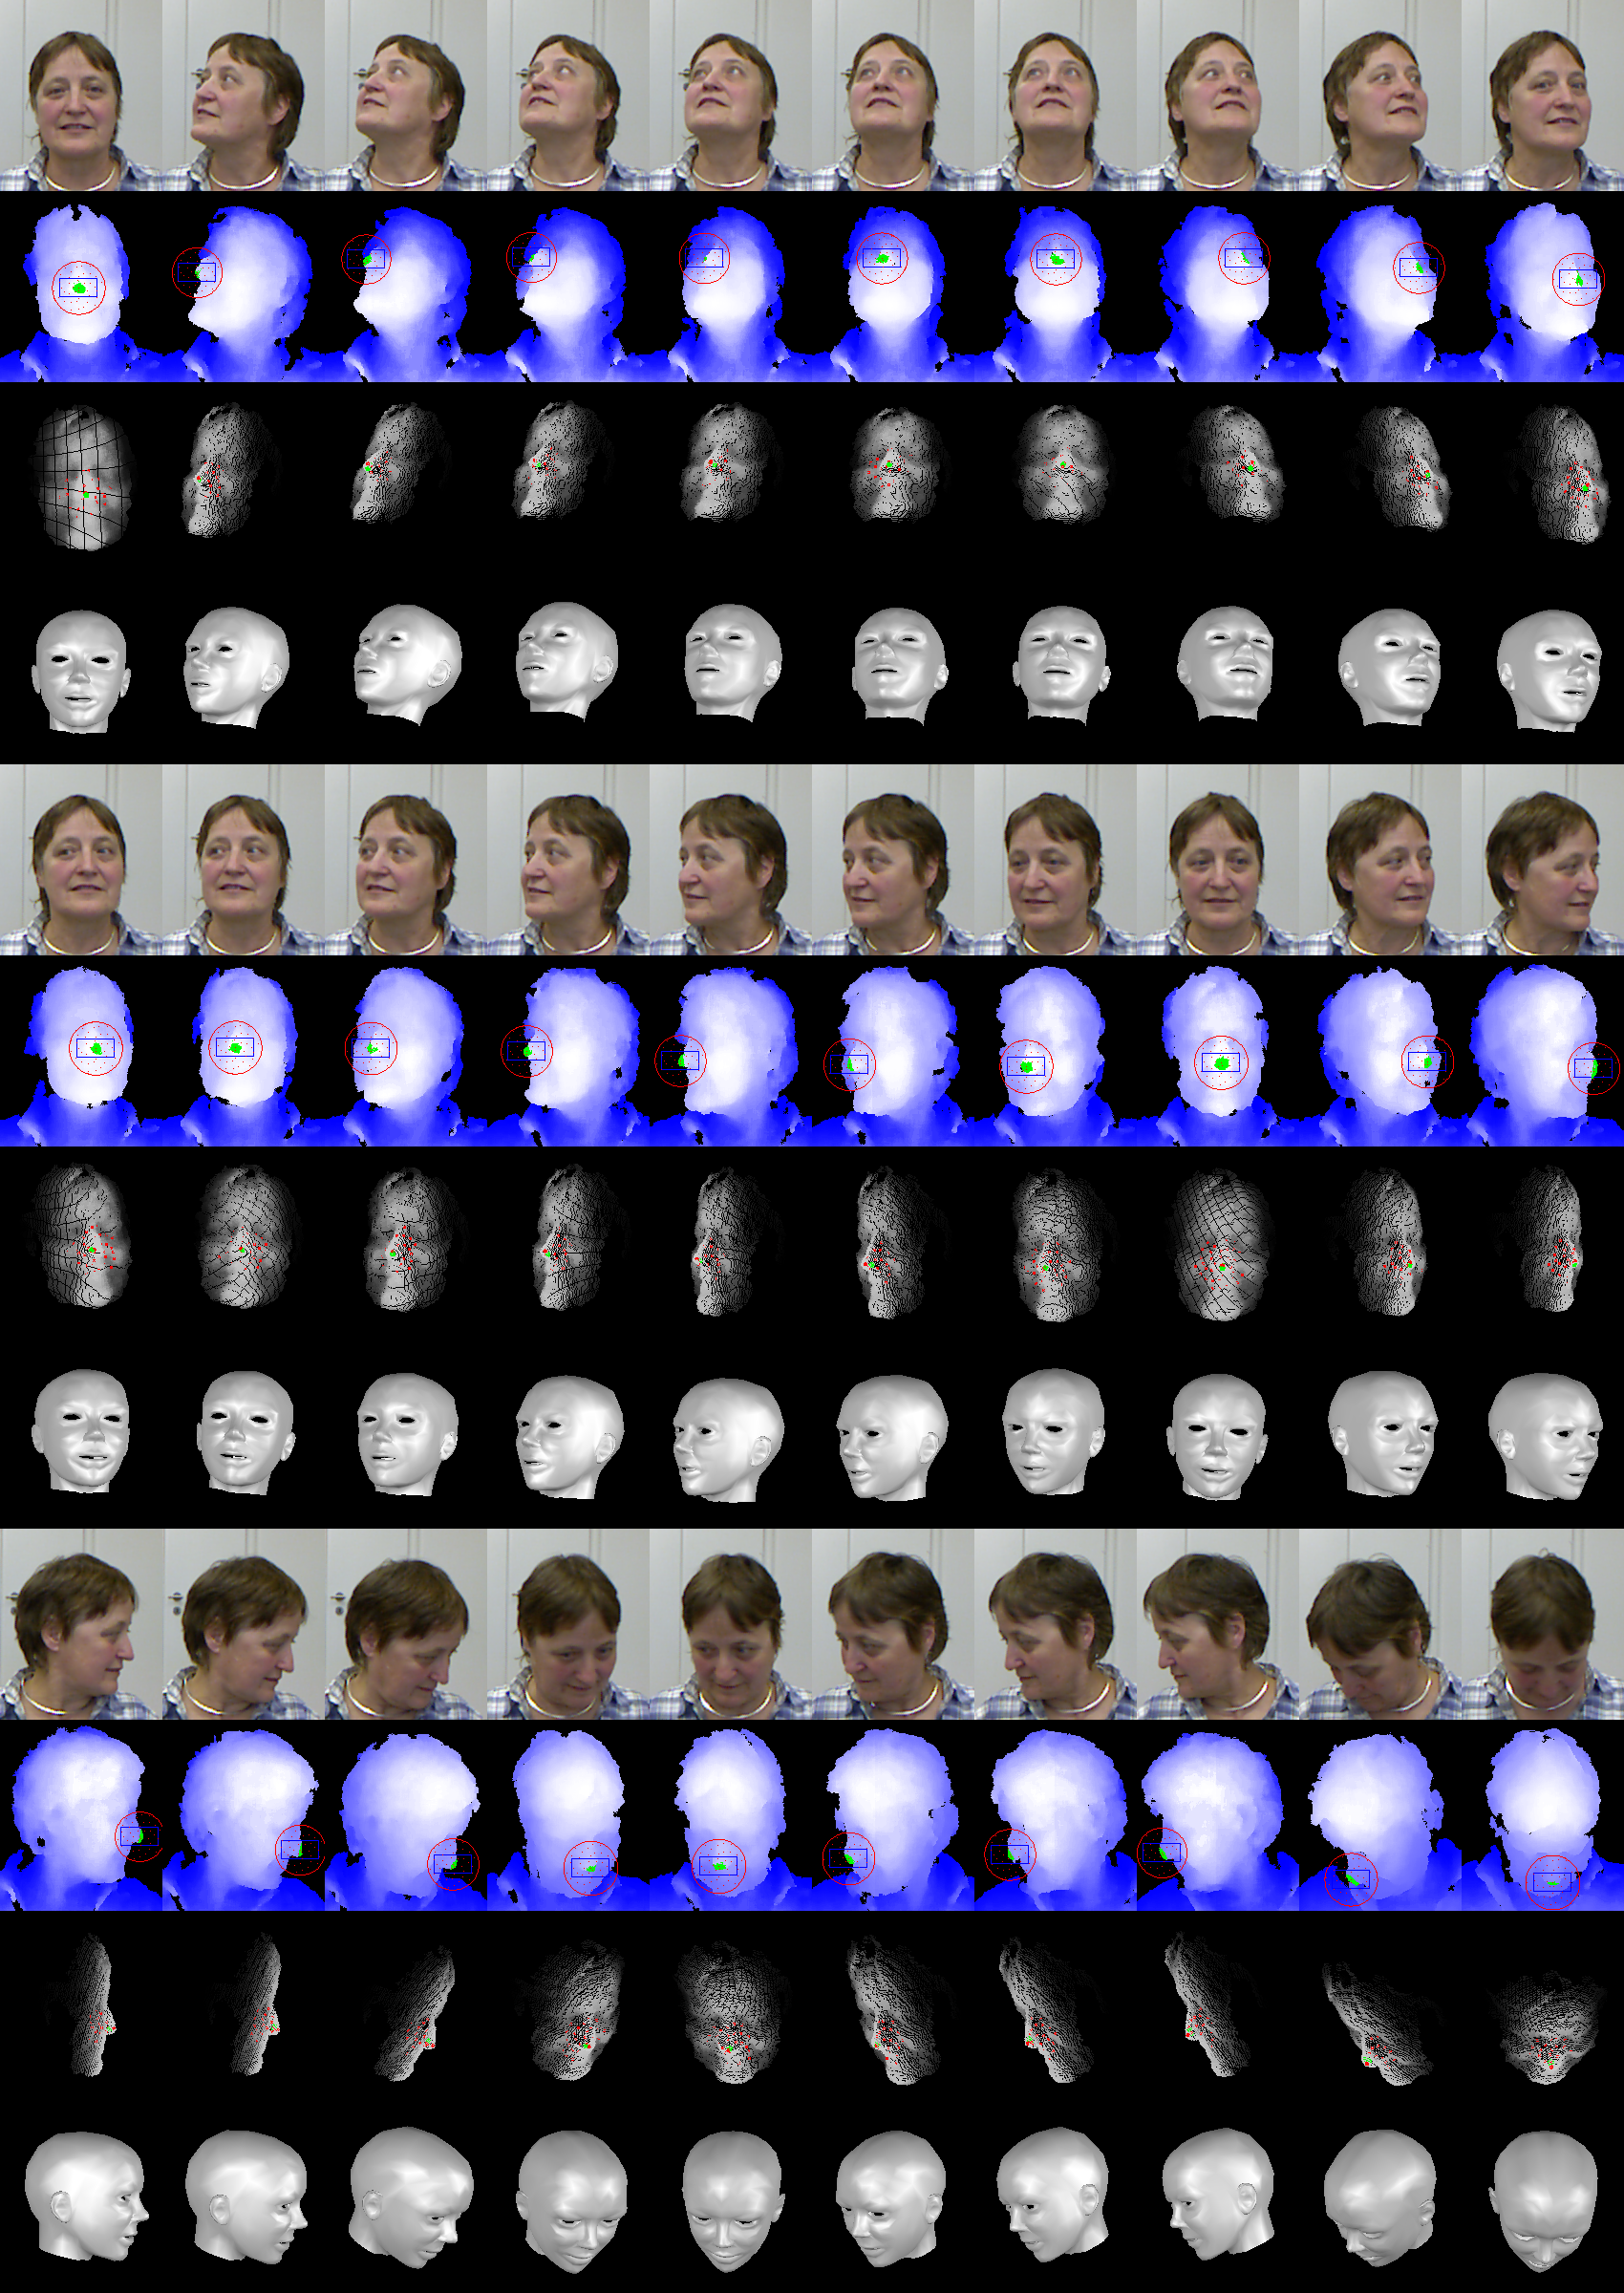
\includegraphics[width=1.0\linewidth]{./figure/biwi_result_01.png}
\caption{Experimental results of optimization solution estimated from one set of BIWI database provided by ETH. The rows of pictures represents user actions, input depth maps, matched results, animated virtual character.}
\label{f:m2 result biwi 01}       % Give a unique label
\end{figure}

\begin{figure}
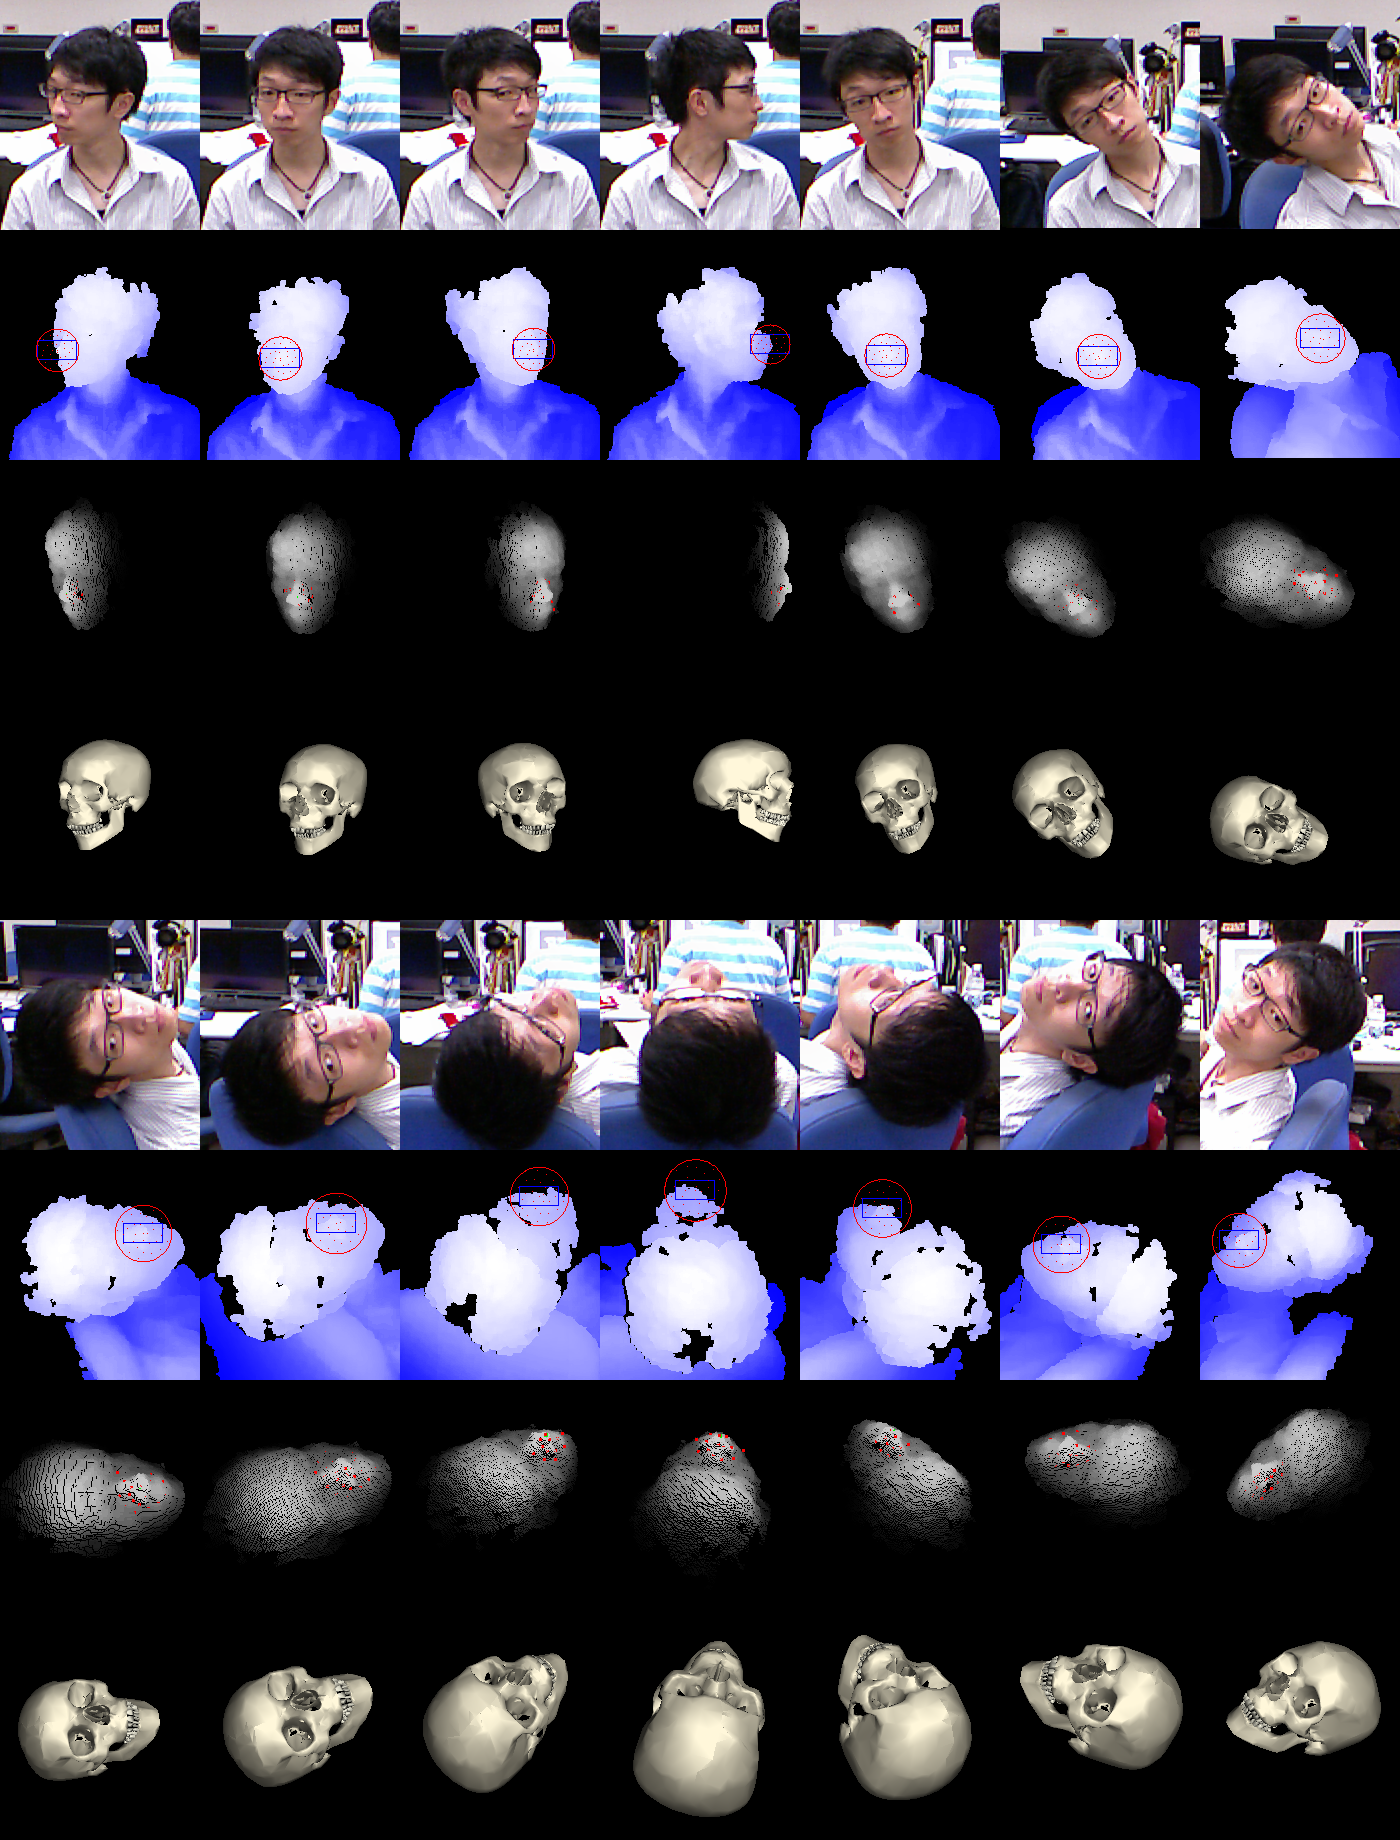
\includegraphics[width=1.0\linewidth]{./figure/Tantofish_Roll_Result.png}
\caption{Experimental results of optimization solution which shows ability of tracking on large roll angles and the combination of 3-DoF rotation anglee.}
\label{f:m2 result tantofish 2}       % Give a unique label
\end{figure}

\begin{figure}
\includegraphics[width=1.0\linewidth]{./figure/Tantofish_Free_Result.png}
\caption{Experimental results of optimization solution. Tracking-based method successfully prevent the system from being affected by other user in the scene.}
\label{f:m2 result tantofish 3}       % Give a unique label
\end{figure}

\begin{figure}
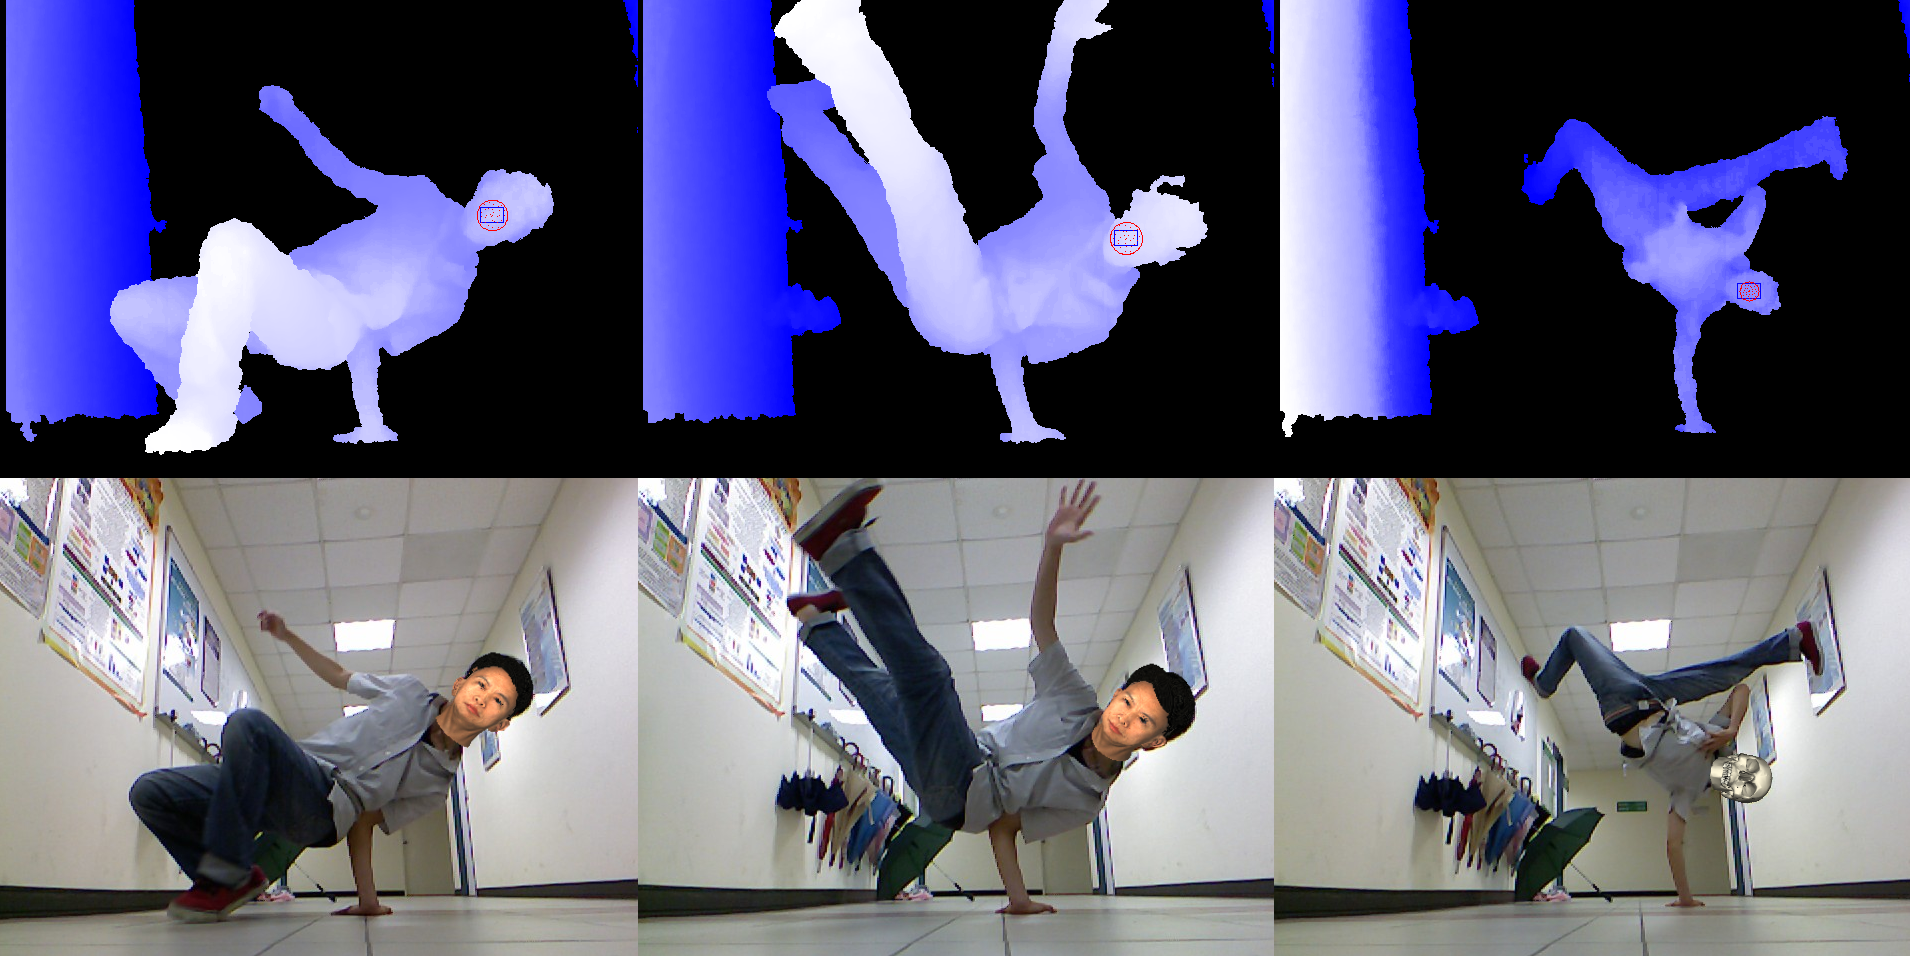
\includegraphics[width=1.0\linewidth]{./figure/StreetDance.png}
\caption{Experimental results of optimization solution - Street dancing.}
\label{f:m2 result tantofish 4}       % Give a unique label
\end{figure}


Figure \ref{f:m2 result tantofish} shows some experimental results of optimization solution (method 2). The first column shows the poses that the user performs. The second column shows the corresponding depth map captured by Kinect. The third column shows the estimated poses. The fourth column overlaps the estimated poses with the observed depth map. Our experiment shows that this method succeeds in estimating the head pose within the range of $\pm 100^{\circ}$ yaw, $\pm 60^{\circ}$ pitch and $\pm 180^{\circ}$ roll rotations. It also shows that this method is more robust and precise than the least square method (method 1). 

Figure \ref{f:m2 result biwi 01} shows more results of the iterative optimization method. These results are estimated from one set of the BIWI database provided by ETH. 

\begin{figure}
\centering
\includegraphics[width=0.5\linewidth]{./figure/ResultCompare.pdf}
\caption{Accuracy of the system in terms of percentage of correctly estimated poses as a function of the angle error threshold using the BIWI database and is compared with \cite{fanelli_DAGM11}}
\label{f:m2 result tantofish 5}       % Give a unique label
\end{figure}


We implement our system on a PC with Intel Core 2 Due CPU P8600 (2.4 GHz), and both of the proposed methods can achieve 30 fps real-time responses.